Survival analysis pertains to data containing survival times, which are \emph{intervals} between certain kinds of events, e.g.; cancer diagnosis date and expiry date. These intervals are often affected by a kind of "partial missingness" called \emph{censoring}. Censored data must be analyzed in a special way to avoid biased estimates and bogus conclusions.
Special methods have been developed long ago to analyze censored data properly.



With survival data, including the SEER data considered in this study, you may not know the exact time of death for some subjects. Some of the SEER subjects are still alive at the the time of the latest SEER data release. When the \codewhite{VITAL STATUS RECODE} variable indicates that the subject is still alive, the \codewhite{SURVIVAL MONTHS} variable is only a lower bound on the true number of survival months; this is called the \textit{date of last contact} mode of censoring. You know that each subject either died on a certain date or was definitely alive up to some last-seen date (and you don't know how far beyond that date he or she may ultimately have lived). The latter situation is called a \textit{censored} observation. 

Statisticians have developed some traditional techniques to utilize the partial information contained in censored observations: the life-table method and the Kaplan-Meier method. 
Both of these methods make use of the partial information to provide unbiased estimates of the two fundamental concepts: - \textit{hazard} and \textit{survival}, both of which are functions of time:

\begin{itemize}[noitemsep]
\item \textbf{The hazard rate} $\lambda(t)$ is the probability of dying in the next small interval of time, assuming that the subject is alive right now.
\item \textbf{The survival rate} $S(t)$  is the probability of living for a certain amount of time after some starting point.
\end{itemize}


Incorrect treatment of survival data still seen in practice, and leading to biased results, includes simply excluding all subjects with a censored survival time from any survival analysis, and \emph{imputing} (replacing) the censored (last-seen) date with some reasonable value. Both of these techniques destroy the partial information contained in the censored observations and nullify the validity of the resulting estimates for the hazard rate and survival rate~\cite{cam}.

In 1958, Edward L. Kaplan and Paul Meier collaborated to publish the seminal paper on how to estimate the hazard and survival rates for data containing censored observations~\cite{Kaplan1958457}.
The method is straightforward and for small datasets can be performed by hand. As an example, consider the survival data shown  in Table~(\ref{tab:censoredexample}). The Kaplan-Meier calculation of the survival curve, the first step is to  
sort the subjects in Table~(\ref{tab:censoredexample}) labeled 0 through 9 by \emph{Survival Time} in ascending order.  
This process results in the first two columns (\emph{Censored Status}, and \emph{Survival Times}) in Table~(\ref{tab:kaplanexample}).
The \emph{At Risk} column decreases by one for each row; in every row a subject has either been censored out of the study or has died. The hazard rate is then computed for each value of \emph{Survival Time} (necessarily a discrete function because the number of subjects is countable), by dividing the value in \emph{Censored Status} by the value in 
\emph{At Risk}. The hazard function is shown in \emph{Prob of Dying} in Table~(\ref{tab:kaplanexample}).
It is then straightforward to calculate the survival function; 1 - hazard function represents the probability of not dying in the next interval of time, assuming that the subject has survived up until now and is represented by column \emph{Prob of Surv}. 
The cumulative survival probability can then be obtained by sucessively multiplying all these individual time-slice probabilities together. In order to survive 2.4 years, first the subject has to survive .5 years, then survive .75 years, 2.3 years and 2.4 years. The probability of surviving 2.4 years is then the product of these 3 probabilities and is given as .666 in Table(\ref{tab:kaplanexample}) in the \emph{Survival Function} column.






\begin{table}[tbp]
\begin{center}
\rowcolors{1}{white}{light-gray}
\begin{tabular}{lrr}
\toprule
{} &  Survival Time (Years) &  Censored Status \\
\midrule
0 &            0.75 &                1 \\
1 &            6.10 &                1 \\
2 &            7.00 &                0 \\
3 &            2.40 &                1 \\
4 &            0.50 &                0 \\
5 &            4.50 &                1 \\
6 &            3.50 &                0 \\
7 &            5.80 &                0 \\
8 &            2.30 &                1 \\
9 &            5.20 &                1 \\
\bottomrule
\end{tabular}
\caption{\label{tab:censoredexample} Example data to illustate traditional Survival Analsyis.}
\end{center}
\end{table}







%To construct a lifetable, one proceeds as follows:




The Kaplan-Meier survival estimate corresponding to the data given in Table~(\ref{tab:censoredexample}) is shown in Table~(\ref{tab:kaplanexample}).

\begin{table}[tbp]
\begin{center}
\rowcolors{1}{white}{light-gray}
\begin{tabular}{lrrrrrr}
\toprule
{} &  Censored Status &  Survival Time &  At Risk &  Prob of Dying &  Prob of Surv & Survival Function \\
\midrule
4 &                0 &            0.50 &              10 &       0.000000 &      1.000000 &      1.000000 \\
0 &                1 &            0.75 &               9 &       0.111111 &      0.888889 &      0.888889 \\
8 &                1 &            2.30 &               8 &       0.125000 &      0.875000 &      0.777778 \\
3 &                1 &            2.40 &               7 &       0.142857 &      0.857143 &      0.666667 \\
6 &                0 &            3.50 &               6 &       0.000000 &      1.000000 &      0.666667 \\
5 &                1 &            4.50 &               5 &       0.200000 &      0.800000 &      0.533333 \\
9 &                1 &            5.20 &               4 &       0.250000 &      0.750000 &      0.400000 \\
7 &                0 &            5.80 &               3 &       0.000000 &      1.000000 &      0.400000 \\
1 &                1 &            6.10 &               2 &       0.500000 &      0.500000 &      0.200000 \\
2 &                0 &            7.00 &               1 &       0.000000 &      1.000000 &      0.200000 \\
\bottomrule
\end{tabular}
\caption{\label{tab:kaplanexample} Kaplan-Meier table corresponding to the example data in Table~(\ref{tab:censoredexample}).}
\end{center}
\end{table}




%%%%%%%%%%%%%%%%%%%%%%%%%%%%%%%%%%%%%%

With just the above data preparation, it is possible to construct traditional Kaplan-Meier estimates of the survival curves for the colon cancer population represented by this subset of the data.
After the above one-hot encoding procedure, the new variable
\codewhite{vital\_status\_recode\_Dead} indicates that the patient is deceased if this variable = 1, or else that the patient's record is right-censored if this variable = 0.
\codewhite{SURVIVAL MONTHS} and \codewhite{vital\_status\_recode\_Dead} are all that is needed to construct the Kaplan-Meier estimate shown in Figure~(\ref{fig:breastkaplan}).

\begin{figure}[tbp]
\centering 
%\begin{center}/\end{center} takes some additional vertical space
%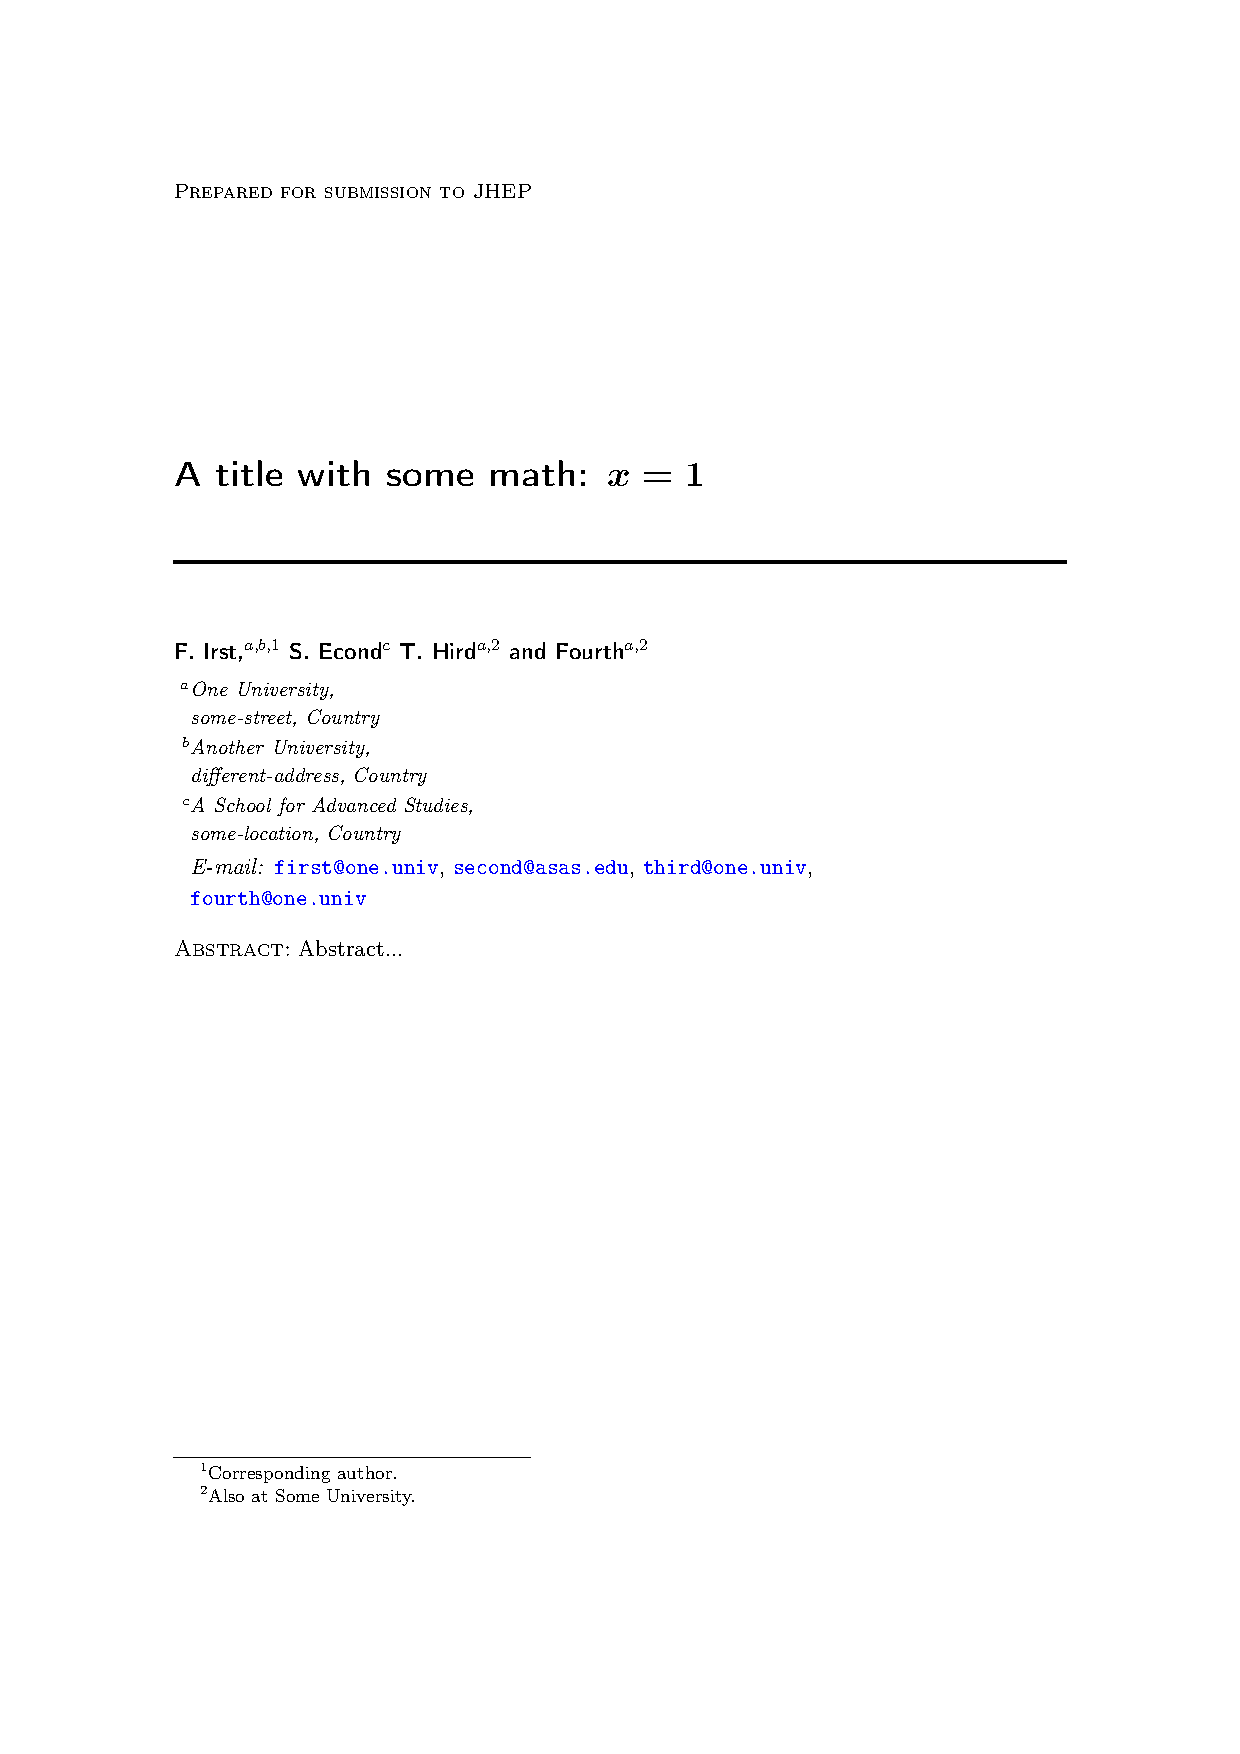
\includegraphics[width=.45\textwidth,trim=0 380 0 200,clip]{img1.pdf}
%\hfill
\begin{center}
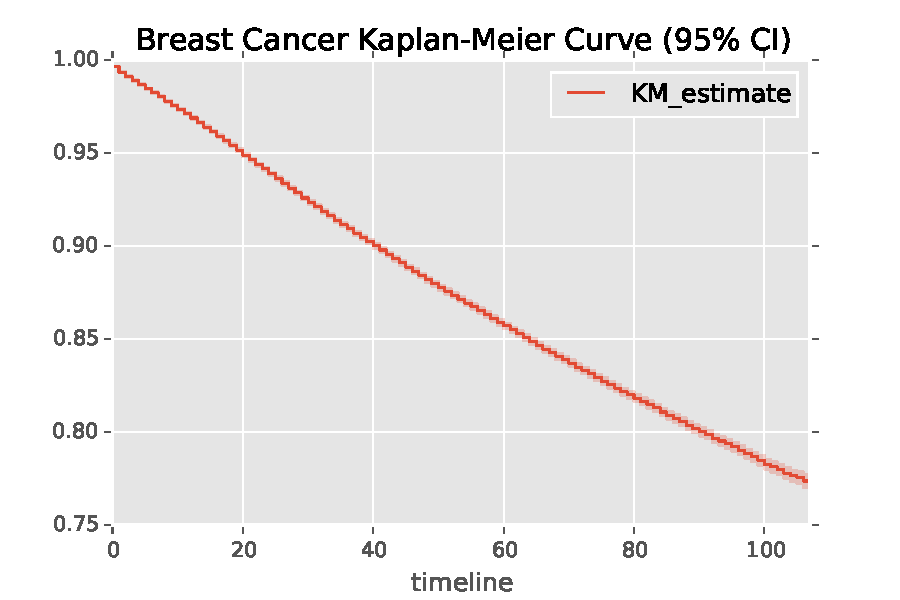
\includegraphics[width=.90\textwidth,origin=c]{breastkaplan.pdf}
% "\includegraphics" is very powerful; the graphicx package is already loaded
\caption{\label{fig:breastkaplan} Traditional Kaplan-Meier estimate of the survival curve for all breast cancer patients. Fitted with 329949 observatins, 292279 censored.}
\end{center}
\end{figure}


\begin{figure}[tbp]
\centering 
%\begin{center}/\end{center} takes some additional vertical space
%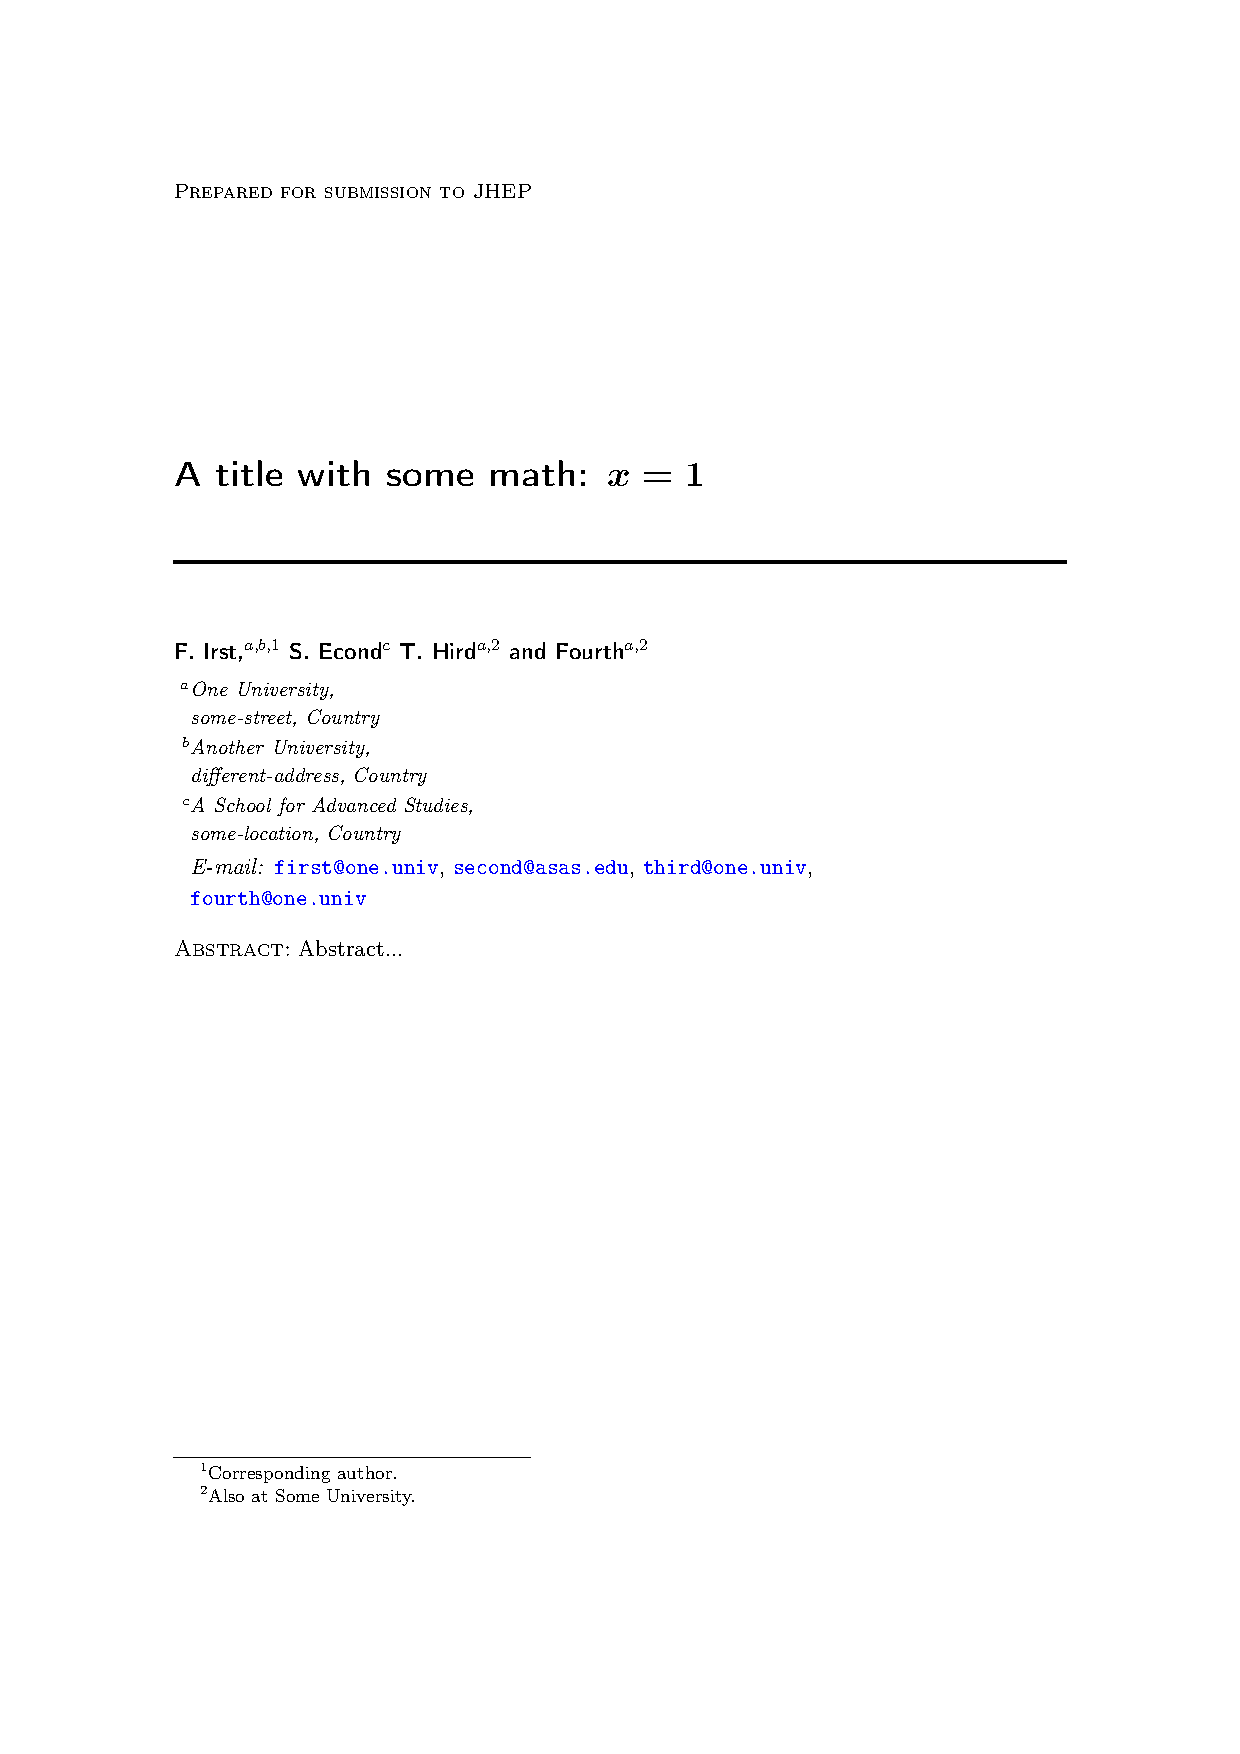
\includegraphics[width=.45\textwidth,trim=0 380 0 200,clip]{img1.pdf}
%\hfill
\begin{center}
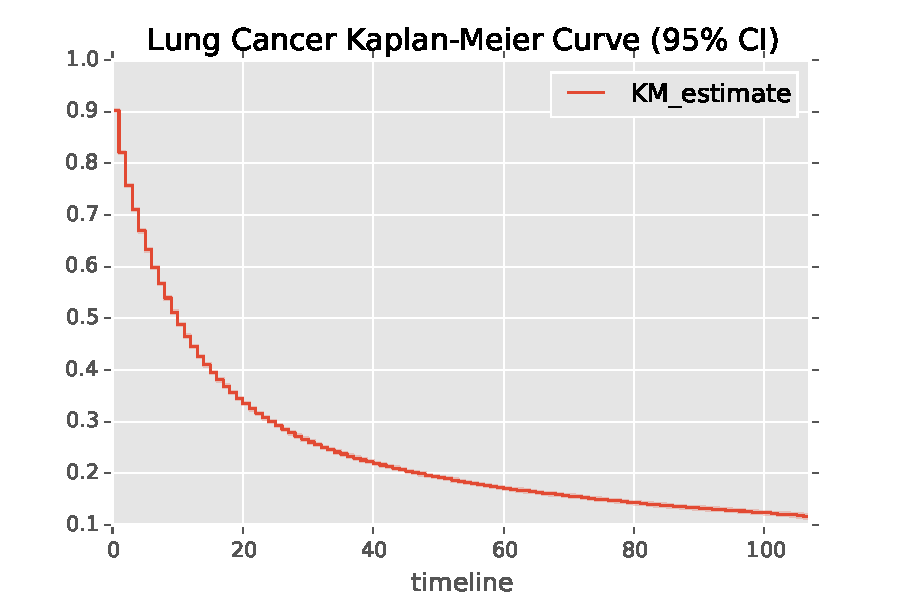
\includegraphics[width=.90\textwidth,origin=c]{lungkaplan.pdf}
% "\includegraphics" is very powerful; the graphicx package is already loaded
\caption{\label{fig:lungkaplan} Traditional Kaplan-Meier estimate of the survival curve for all lung cancer patients. Fitted with 177089 observatins, 47409 censored.}
\end{center}
\end{figure}



The above Kaplan-Meier estimates of the survival curves for colon (Figure~(\ref{fig:colonkaplan})), lung 
(Figure~(\ref{fig:lungkaplan})), and breast cancer (Figure~(\ref{fig:breastkaplan})) are constructed from the full population of cancer patients in the respective datasets.
An unsatisfactory consequence is that these estimates are highly course-grained, and not very meaningful to an indivual. Patients with very disparate characteristics are given the same prognosis by these Kaplan-Meier survival curve estimates. Therefore it is desirable to find robust predictors for survival curves of individual subjects where the input is an individual record as opposed to a population. In section~(\ref{subsec:transformation}) we present the data transformation that allows for machine learning to be applied to censored data.



